\chapter{Extrapolation of difference quotients}

\section{The algorithm}

Let \(a\in \R\), \(\varepsilon > 0\) and \(f:]a - \varepsilon, a + \varepsilon [ \rightarrow \R\) be differentiable at \(a\). We are interested in estimating \(f'(a)\). Assume that \(f\) is \(2k+1\) times differentiable at \(a\). Then by Taylor's theorem we have 
\begin{equation}\label{taylor}
f(a + h) = f(a) + f'(a)h + \frac{f''(a)}{2}h^2 + \cdots + \frac{f^{(2k)}(a)}{(2k)!}h^{2k} + \frac{f^{(2k+1)}(\xi)}{(2k+1)!}h^{2k+1}
\end{equation}
where \(a < \xi < a + h\). Now plug \(-h\) instead of \(h\) in (\ref{taylor}):
\begin{equation}\label{taylorm}
f(a-h) = f(a) - f'(a)h + \frac{f''(a)}{2}h^2 - \cdots + \frac{f^{(2k)}(a)}{(2k)!}h^{2k} -  \frac{f^{(2k+1)}(\eta)}{(2k+1)!}h^{2k+1}
\end{equation}
where \(a - h < \eta < a\). If we subtract (\ref{taylorm}) from (\ref{taylor}) and divide by \(2h\) we get:
\begin{equation}\label{middlestep}
f'(a) = D_f(h) + \frac{f'''(a)}{3!}h^2 + \cdots + \frac{f^{(2k-1)}(a)}{(2k-1)!}h^{2k-2} + \frac{f^{(2k+1)}(\xi) + f^{(2k+1)}(\eta)}{2\cdot (2k+1)!}h^{2k}
\end{equation}
where
\begin{equation}
D_f(h) \coloneqq \frac{f(a+h) - f(a-h)}{2h}
\end{equation}
is the {\it symmetric difference quotient} of \(f\) at \(a\). Note that \(\frac{1}{2}(f^{(2k+1)}(\xi) + f^{(2k+1)}(\eta))\) is in the image of \(f^{(2k+1)}\) so we can rewrite (\ref{middlestep}) as 
\begin{equation}\label{symmdiff}
f'(a) = D_f(h) + \frac{f'''(a)}{3!}h^2 + \cdots + \frac{f^{(2k-1)}(a)}{(2k-1)!}h^{2k-2} + \frac{f^{(2k+1)}(\zeta)}{(2k+1)!}h^{2k}
\end{equation}
where \(a-h < \zeta < a + h\). Formula (\ref{symmdiff}) tells us that the symmetric difference quotient method has asymptotic expansion in \(h^2\) of order \(2k-2\) if \(f\) is \(2k+1\) times differentiable. Thus we can use the following scheme to extrapolate the symmetric difference quotient method:

\begin{enumerate}
    \item \(D_{i1} \coloneqq D_f(h_i)\) for \(i = 1,\ldots,k\).
    \item \(D_{ij} \coloneqq D_{i,j-1} + \frac{D_{i,j-1} - D_{i-1,j-1}}{\left(\frac{h_{i-j+1}}{h_i}\right)^2 - 1}\) for \(2\leq j\leq i\).
\end{enumerate}

\section{Numerical experiments}

In this section we are going to extrapolate the symmetric difference quotient for approximating the derivative of a function at a given point. Let \(h > 0\) be some number, \(f: ]a-\varepsilon, a+\varepsilon[\rightarrow \R\) a function differentiable at \(a\) and \(n_1 < n_2 < \cdots\) a sequence of integers. Let \(h_i \coloneqq h/n_i\). Let \(D_{ij}\) be the extrapolation table that we get from extrapolating in \(h^2\) using the points \((h_1^2,D_f(h_1)),(h_2^2,D_f(h_2)),\ldots\), as we described in the first chapter. We let \(\varepsilon_i \coloneqq |X_{ii} - f'(a)|\). We want to analyse how \(\varepsilon_i\) as \(i\) increases and we also want to do similar efficiency analysis as in the chapter on Romberg quadrature and check whether we have exponential convergence. We will do the computations with precision up to \(500\) significant digits and also using standard double precision arithmetic.\\

Now we will consider the results of the experiments.

\subsection{The exponential function}

We begin by considering the derivative of the exponential function at zero. 

\begin{figure}[H]
\centering
\begin{minipage}{0.45\textwidth}
\centering
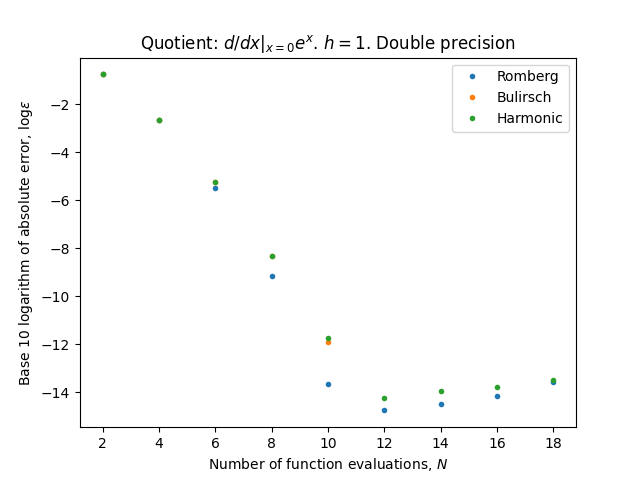
\includegraphics[scale=0.45]{../results/diff_quot_plots/exp_0.png}
\end{minipage}
\begin{minipage}{0.45\textwidth}
\centering
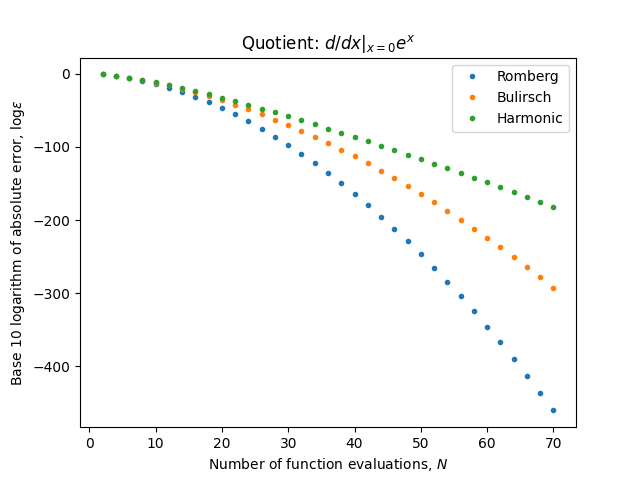
\includegraphics[scale=0.45]{../results/diff_quot_plots/exp_0_hp.png}
\end{minipage}
\end{figure}

\begin{figure}[H]
\centering
\begin{minipage}{0.45\textwidth}
\centering
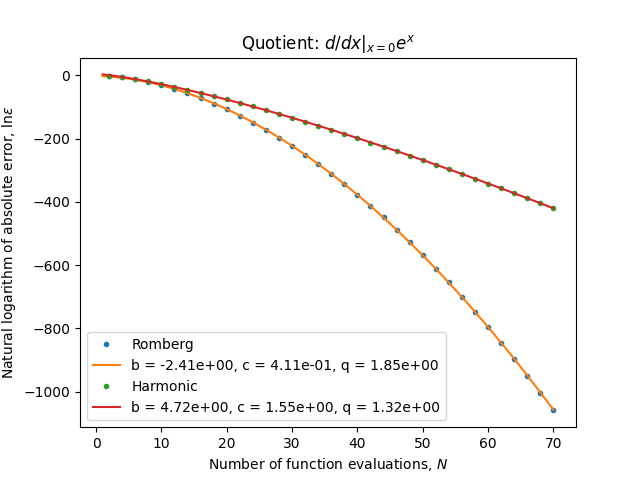
\includegraphics[scale=0.45]{../results/diff_quot_plots/exp_0_hp_trend.png}
\end{minipage}
\begin{minipage}{0.45\textwidth}
\centering
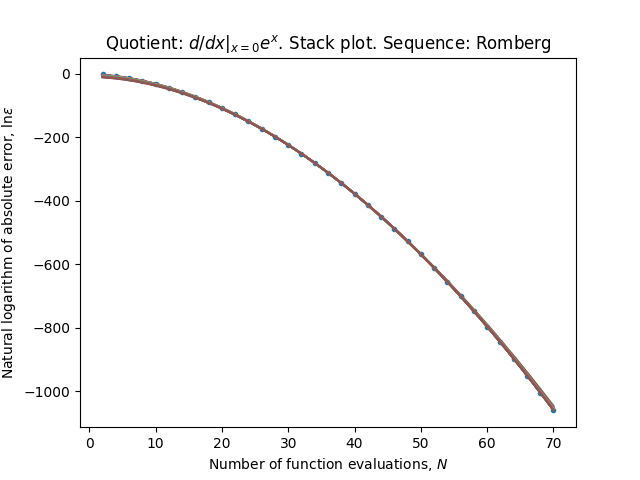
\includegraphics[scale=0.45]{../results/diff_quot_plots/exp_0_hp_romberg_stack.png}
\end{minipage}
\end{figure}

\begin{figure}[H]
\centering
\begin{minipage}{0.45\textwidth}
\centering
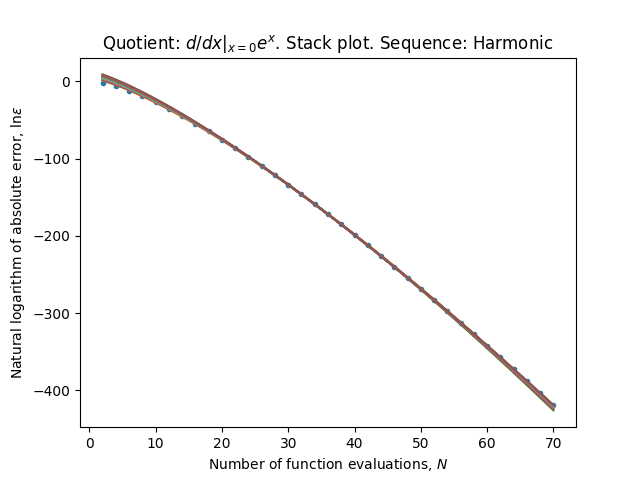
\includegraphics[scale=0.45]{../results/diff_quot_plots/exp_0_hp_harmonic_stack.png}
\end{minipage}
\end{figure}

\begin{table}[H]
    \centering
    \small
    \begin{tabular}{c||c|c|c|c|c|c|c|c}
Sequence & \(A\)-mean & \(A\)-var & \(c\)-mean & \(c\)-var & \(q\)-mean & \(q\)-var & \(\rho_{\operatorname{lin}}\) & \(\rho_{\ln}\)\\\hline
\rowcolor{green}
RS & \(3.7[-02]\) & \(2.6[+00]\) & \(4.0[-01]\) & \(4.0[-03]\) & \(1.9[+00]\) & \(6.7[-05]\) & \(7.8[-01]\) & \(3.0[-06]\) \\
\rowcolor{green}
HS & \(1.1[+05]\) & \(3.3[+00]\) & \(1.7[+00]\) & \(7.2[-03]\) & \(1.3[+00]\) & \(2.4[-04]\) & \(1.5[+02]\) & \(1.2[-05]\) \\
    \end{tabular}
    \label{tab:my_label}
\end{table}

In standard floating point arithmetic, we get down to machine level precision using any sequence. The Romberg sequence works best, then Bulirsch and then the harmonic. The model seems to fit well in all cases.

\subsection{Logarithm}

Now we will consider the dervative at zero of the function 
\[
g(x) \coloneqq \ln(x+1).
\]

\begin{figure}[H]
\centering
\begin{minipage}{0.45\textwidth}
\centering
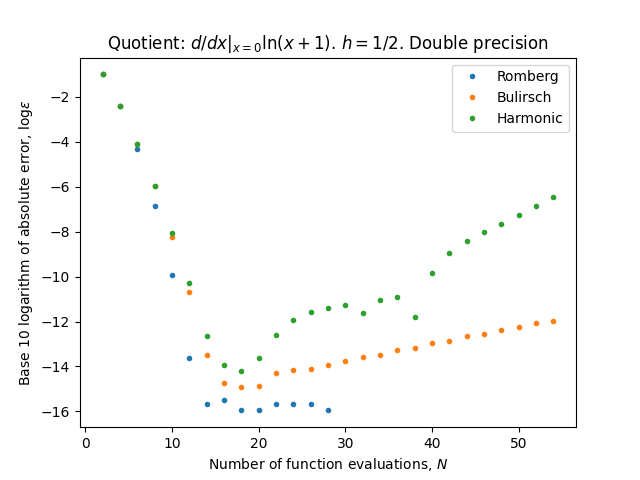
\includegraphics[scale=0.45]{../results/diff_quot_plots/h_one.png}
\end{minipage}
\begin{minipage}{0.45\textwidth}
\centering
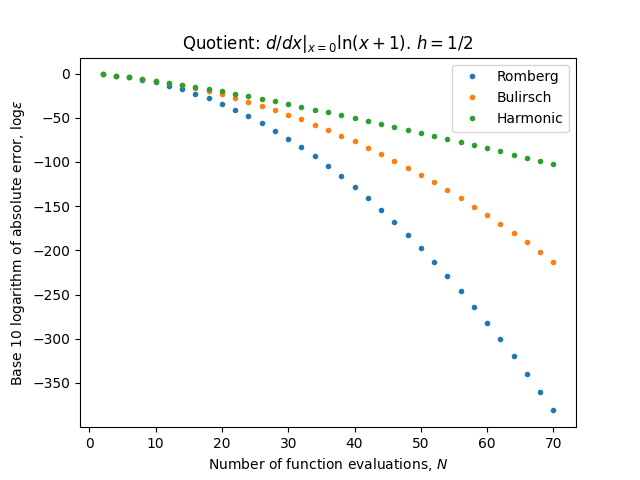
\includegraphics[scale=0.45]{../results/diff_quot_plots/h_one_hp.png}
\end{minipage}
\end{figure}

\begin{figure}[H]
\centering
\begin{minipage}{0.45\textwidth}
\centering
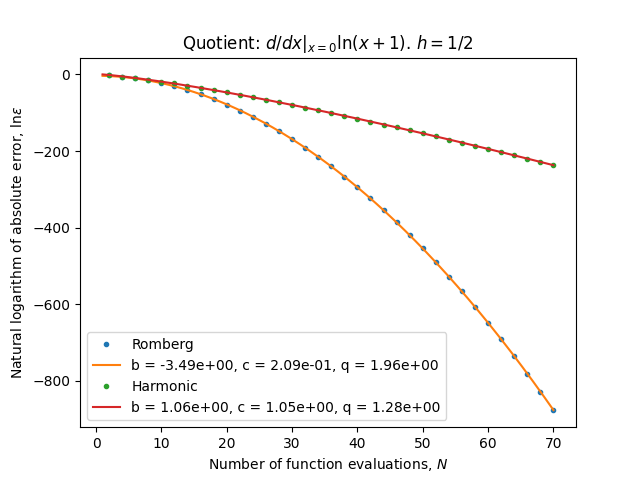
\includegraphics[scale=0.45]{../results/diff_quot_plots/h_one_hp_trend.png}
\end{minipage}
\begin{minipage}{0.45\textwidth}
\centering
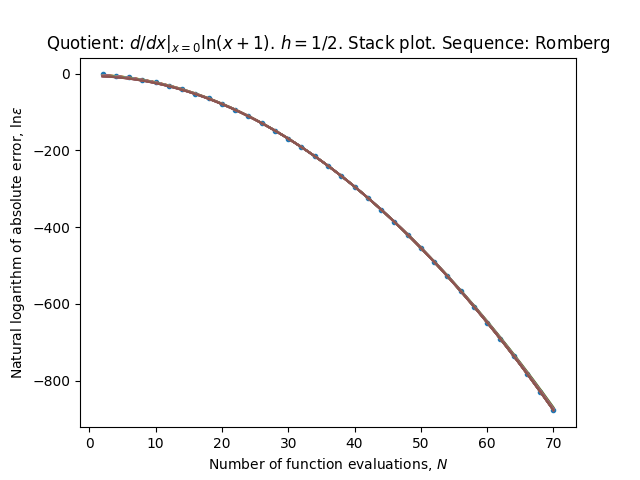
\includegraphics[scale=0.45]{../results/diff_quot_plots/h_one_hp_romberg_stack.png}
\end{minipage}
\end{figure}

\begin{figure}[H]
\centering
\begin{minipage}{0.45\textwidth}
\centering
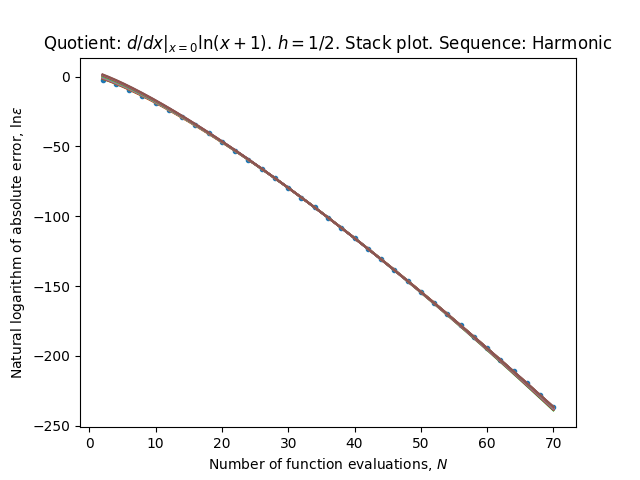
\includegraphics[scale=0.45]{../results/diff_quot_plots/h_one_hp_harmonic_stack.png}
\end{minipage}
\end{figure}

\begin{table}[H]
    \centering
    \small
    \begin{tabular}{c||c|c|c|c|c|c|c|c}
Sequence & \(A\)-mean & \(A\)-var & \(c\)-mean & \(c\)-var & \(q\)-mean & \(q\)-var & \(\rho_{\operatorname{lin}}\) & \(\rho_{\ln}\)\\\hline
\rowcolor{green}
RS & \(9.1[-03]\) & \(9.8[-01]\) & \(2.0[-01]\) & \(1.4[-03]\) & \(2.0[+00]\) & \(2.1[-05]\) & \(7.5[-01]\) & \(2.1[-06]\) \\
\rowcolor{green}
HS & \(2.8[+01]\) & \(9.6[-01]\) & \(1.1[+00]\) & \(3.5[-03]\) & \(1.3[+00]\) & \(1.2[-04]\) & \(1.7[+00]\) & \(4.5[-06]\) \\
    \end{tabular}
    \label{tab:my_label}
\end{table}

We get down to machine level precision using any sequence, Romberg performes best, then Bulirsch and then the Harmonic one. The model fits well in all cases.

\subsection{Square root}

Now we shall consider the derivative at zero of the following function:
\[
h(x) \coloneqq \sqrt{1 + x}
\]

\begin{figure}[H]
\centering
\begin{minipage}{0.45\textwidth}
\centering
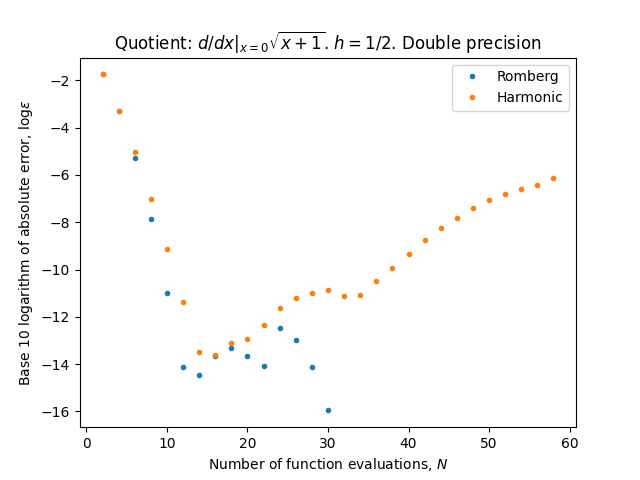
\includegraphics[scale=0.45]{../results/diff_quot_plots/sqrt_1.png}
\end{minipage}
\begin{minipage}{0.45\textwidth}
\centering
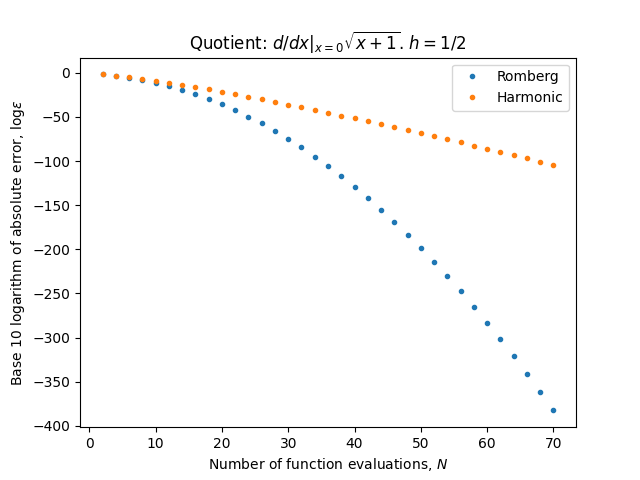
\includegraphics[scale=0.45]{../results/diff_quot_plots/sqrt_1_hp.png}
\end{minipage}
\end{figure}

\begin{figure}[H]
\centering
\begin{minipage}{0.45\textwidth}
\centering
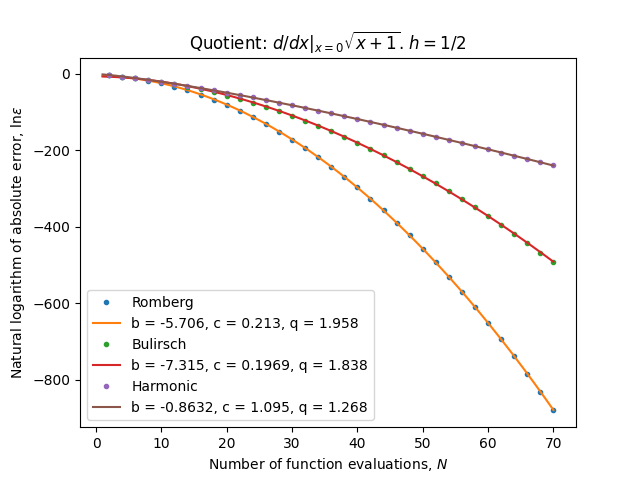
\includegraphics[scale=0.45]{../results/diff_quot_plots/sqrt_1_hp_trend.png}
\end{minipage}
\begin{minipage}{0.45\textwidth}
\centering
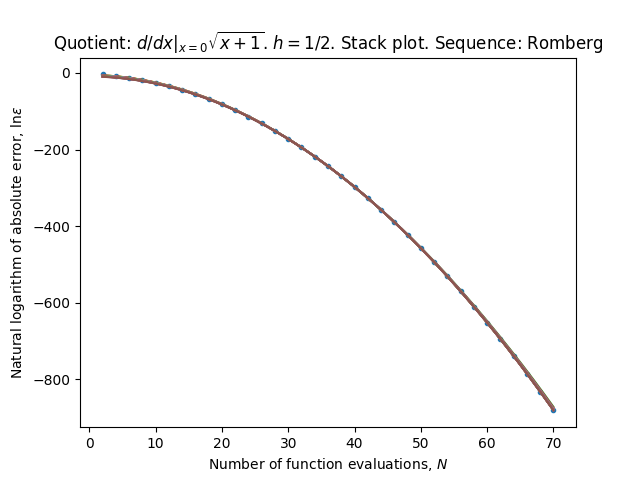
\includegraphics[scale=0.45]{../results/diff_quot_plots/sqrt_1_hp_romberg_stack.png}
\end{minipage}
\end{figure}

\begin{figure}[H]
\centering
\begin{minipage}{0.45\textwidth}
\centering
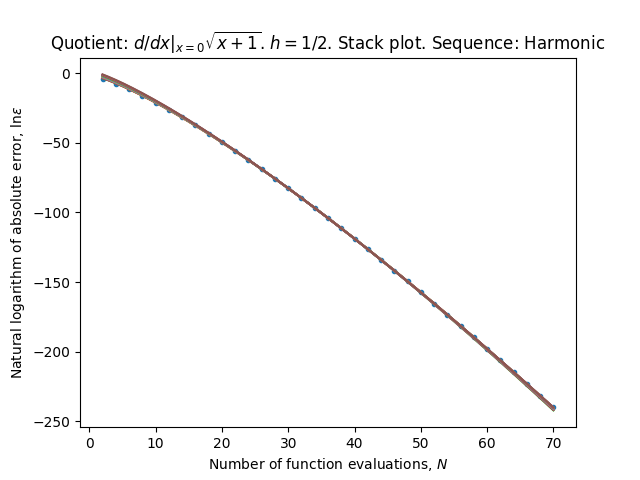
\includegraphics[scale=0.45]{../results/diff_quot_plots/sqrt_1_hp_harmonic_stack.png}
\end{minipage}
\end{figure}

\begin{table}[H]
    \centering
    \small
    \begin{tabular}{c||c|c|c|c|c|c|c|c}
Sequence & \(A\)-mean & \(A\)-var & \(c\)-mean & \(c\)-var & \(q\)-mean & \(q\)-var & \(\rho_{\operatorname{lin}}\) & \(\rho_{\ln}\)\\\hline
\rowcolor{green}
RS & \(8.3[-04]\) & \(1.3[+00]\) & \(2.1[-01]\) & \(1.8[-03]\) & \(2.0[+00]\) & \(2.7[-05]\) & \(8.4[-01]\) & \(2.9[-06]\) \\
\rowcolor{red}
HS & \(2.6[+00]\) & \(8.2[-01]\) & \(1.2[+00]\) & \(2.7[-03]\) & \(1.3[+00]\) & \(8.9[-05]\) & \(5.0[-01]\) & \(2.5[-06]\) \\
    \end{tabular}
    \label{tab:my_label}
\end{table}

In standard double precision floating point arithmetic we get down to machine level precision using any sequence. The model fits well in all cases.

\subsection{Smooth but not analytic function}

Now we will consider the derivate at zero of the following function:
\[
r(x) \coloneqq \begin{cases}
e^{-1/x} & \text{if } x > 0\\
0 & \text{else}
\end{cases}
\]
which is smooth but not analytic.

\begin{figure}[H]
\centering
\begin{minipage}{0.45\textwidth}
\centering
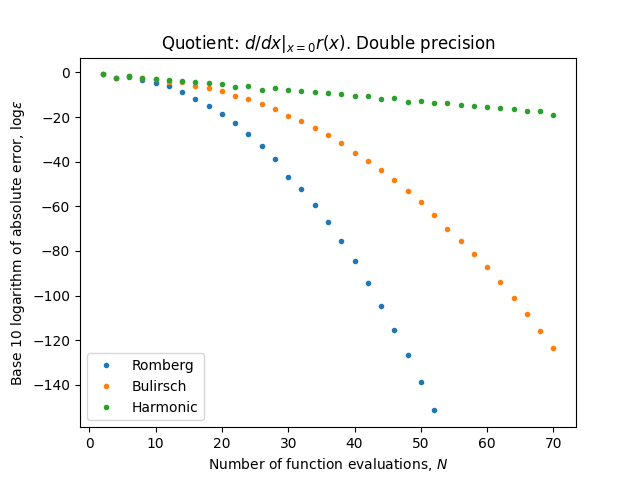
\includegraphics[scale=0.45]{../results/diff_quot_plots/rho.png}
\end{minipage}
\begin{minipage}{0.45\textwidth}
\centering
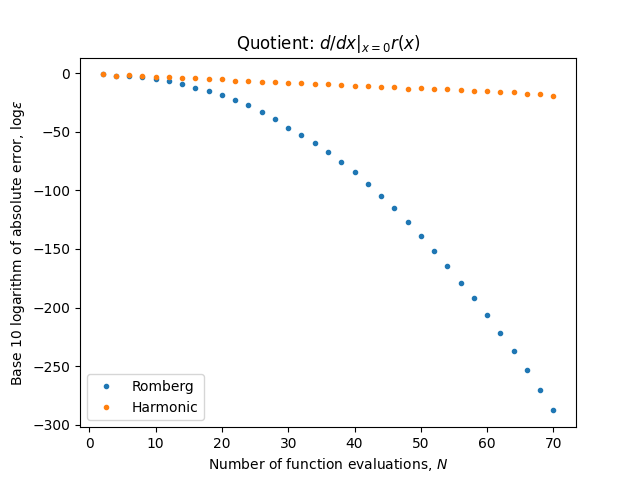
\includegraphics[scale=0.45]{../results/diff_quot_plots/rho_hp.png}
\end{minipage}
\end{figure}

\begin{figure}[H]
\centering
\begin{minipage}{0.45\textwidth}
\centering
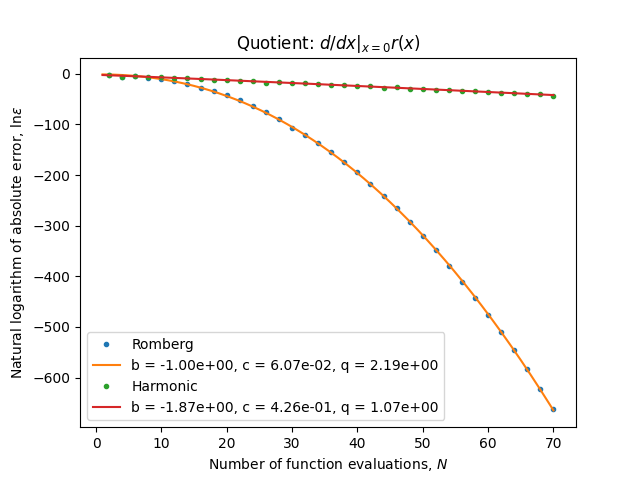
\includegraphics[scale=0.45]{../results/diff_quot_plots/rho_hp_trend.png}
\end{minipage}
\begin{minipage}{0.45\textwidth}
\centering
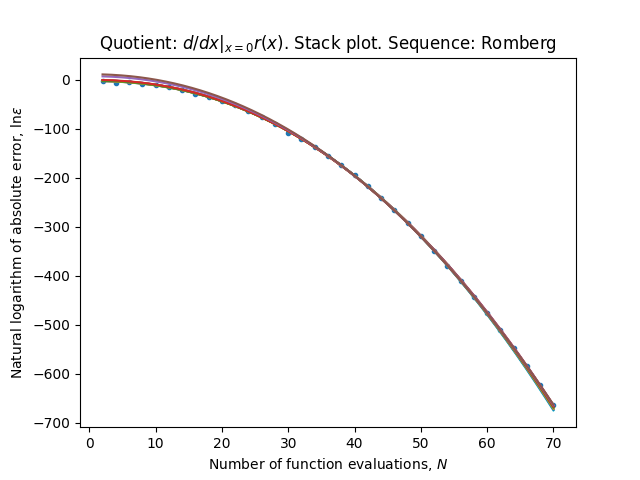
\includegraphics[scale=0.45]{../results/diff_quot_plots/rho_hp_romberg_stack.png}
\end{minipage}
\end{figure}

\begin{figure}[H]
\centering
\begin{minipage}{0.45\textwidth}
\centering
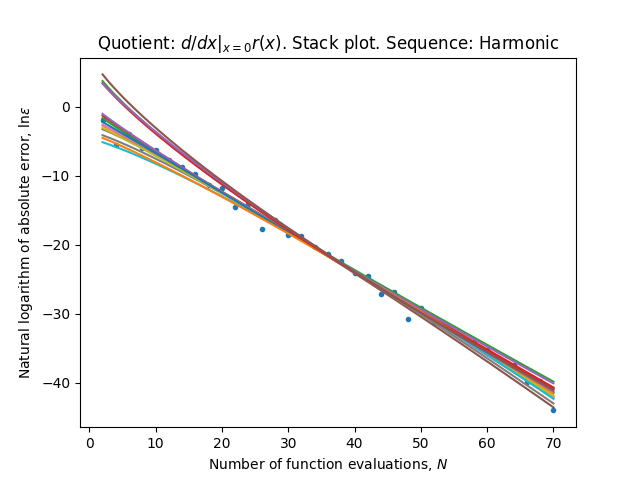
\includegraphics[scale=0.45]{../results/diff_quot_plots/rho_hp_harmonic_stack.png}
\end{minipage}
\end{figure}

\begin{table}[H]
    \centering
    \small
    \begin{tabular}{c||c|c|c|c|c|c|c|c}
Sequence & \(A\)-mean & \(A\)-var & \(c\)-mean & \(c\)-var & \(q\)-mean & \(q\)-var & \(\rho_{\operatorname{lin}}\) & \(\rho_{\ln}\)\\\hline
\rowcolor{green}
RS & \(7.3[+03]\) & \(1.3[+01]\) & \(6.0[-02]\) & \(2.3[-02]\) & \(2.2[+00]\) & \(2.1[-04]\) & \(1.7[+00]\) & \(2.2[-05]\) \\
\rowcolor{red}
HS & \(2.9[+02]\) & \(4.8[+00]\) & \(8.2[-01]\) & \(4.8[-01]\) & \(9.8[-01]\) & \(2.3[-02]\) & \(3.1[-01]\) & \(1.2[-03]\) \\
    \end{tabular}
    \label{tab:my_label}
\end{table}

Romberg performes better.\\

The model seems to fit reasonably well for the Romberg and Bulirsch sequence but the fitting is not so nice for the harmonic sequence.

\subsection{Another smooth but not analytic function}

Now we will consider the derivative at zero of the following function:
\[
i(x)\coloneqq \begin{cases}
xe^{-1/x^2} & \text{if } x \neq 0\\
0 & \text{else}
\end{cases}
\]
which is smooth but not analytic.

\begin{figure}[H]
\centering
\begin{minipage}{0.45\textwidth}
\centering
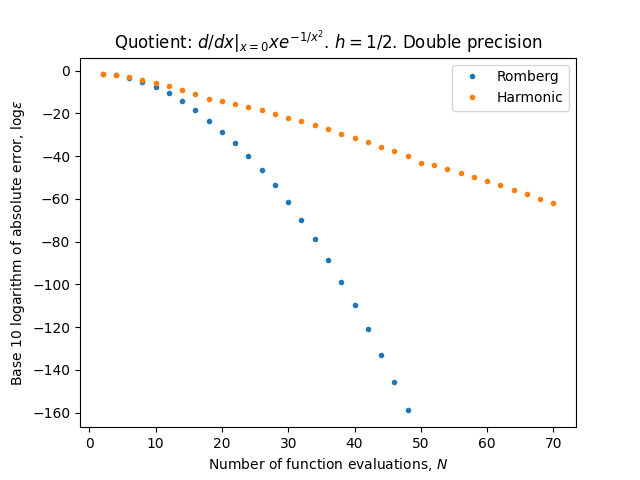
\includegraphics[scale=0.45]{../results/diff_quot_plots/xemxm2.png}
\end{minipage}
\begin{minipage}{0.45\textwidth}
\centering
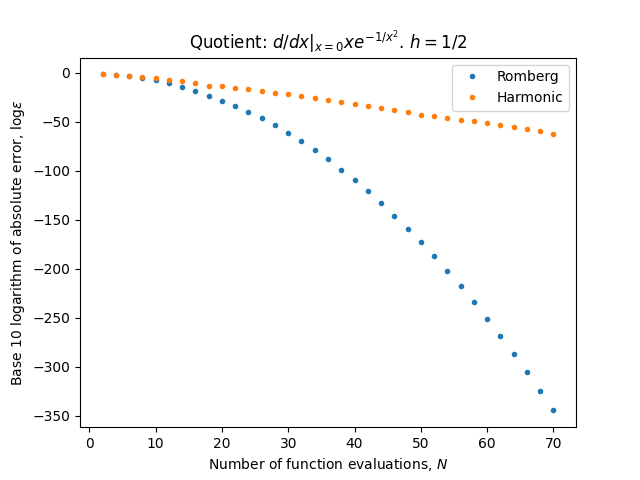
\includegraphics[scale=0.45]{../results/diff_quot_plots/xemxm2_hp.png}
\end{minipage}
\end{figure}

\begin{figure}[H]
\centering
\begin{minipage}{0.45\textwidth}
\centering
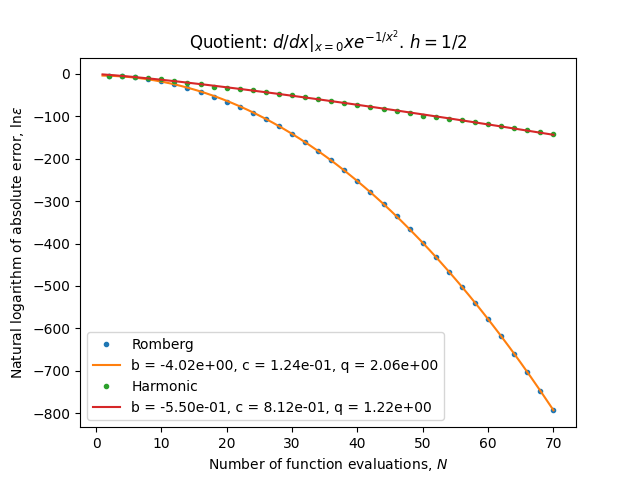
\includegraphics[scale=0.45]{../results/diff_quot_plots/xemxm2_hp_trend.png}
\end{minipage}
\begin{minipage}{0.45\textwidth}
\centering
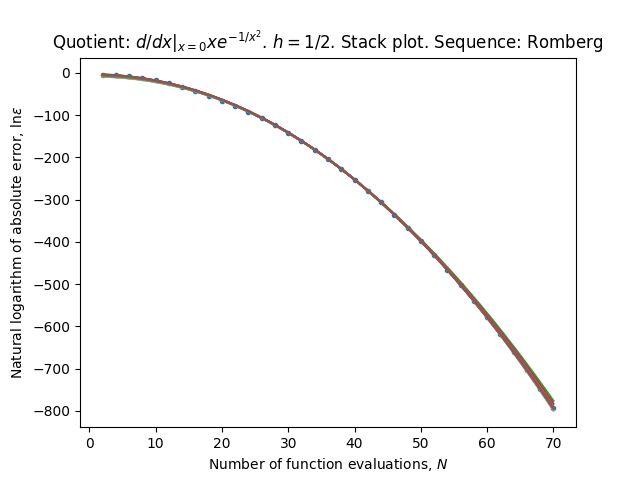
\includegraphics[scale=0.45]{../results/diff_quot_plots/xemxm2_hp_romberg_stack.png}
\end{minipage}
\end{figure}

\begin{figure}[H]
\centering
\begin{minipage}{0.45\textwidth}
\centering
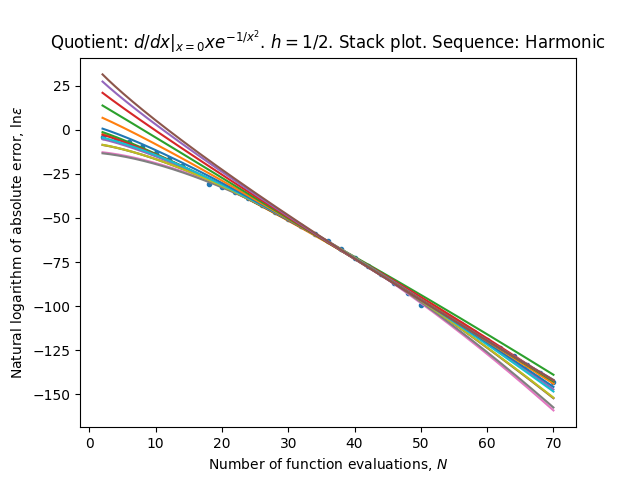
\includegraphics[scale=0.45]{../results/diff_quot_plots/xemxm2_hp_harmonic_stack.png}
\end{minipage}
\end{figure}

\begin{table}[H]
    \centering
    \small
    \begin{tabular}{c||c|c|c|c|c|c|c|c}
Sequence & \(A\)-mean & \(A\)-var & \(c\)-mean & \(c\)-var & \(q\)-mean & \(q\)-var & \(\rho_{\operatorname{lin}}\) & \(\rho_{\ln}\)\\\hline
\rowcolor{green}
RS & \(9.2[-03]\) & \(1.7[+00]\) & \(1.2[-01]\) & \(7.0[-03]\) & \(2.1[+00]\) & \(9.6[-05]\) & \(2.0[-01]\) & \(4.4[-06]\) \\
\rowcolor{red}
HS & \(2.1[+16]\) & \(1.3[+01]\) & \(1.5[+00]\) & \(1.0[+00]\) & \(1.2[+00]\) & \(3.7[-02]\) & \(1.3[+01]\) & \(1.8[-04]\) \\
    \label{tab:my_label}
\end{table}

Here the Romberg sequence performes better.\\

We seem to have nice fit for the Romberg sequence, moderately good for the Bulirsch sequence but not so good for the harmonic sequence.

\subsection{Only once differentiable function}

Finally we will consider the derivate at zero of the following function which is only once differentiable at that point:
\[
j(x)\coloneqq \begin{cases}
x^2\sin\frac{1}{x} & \text{if } x \neq 0\\
0 & \text{else}
\end{cases}.
\]

\begin{figure}[H]
\centering
\begin{minipage}{0.45\textwidth}
\centering
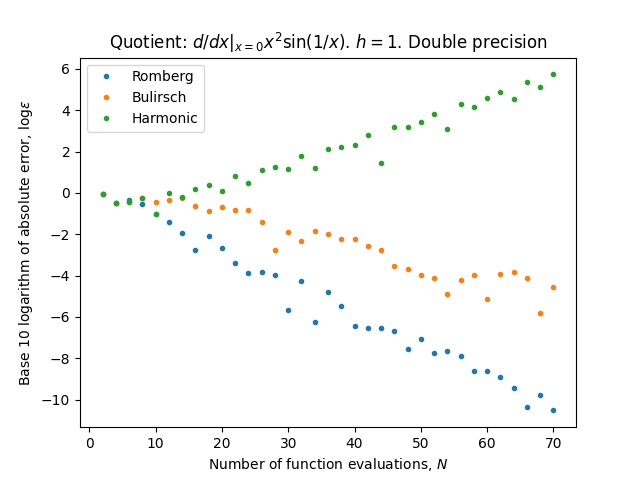
\includegraphics[scale=0.45]{../results/diff_quot_plots/xsin.png}
\end{minipage}
\begin{minipage}{0.45\textwidth}
\centering
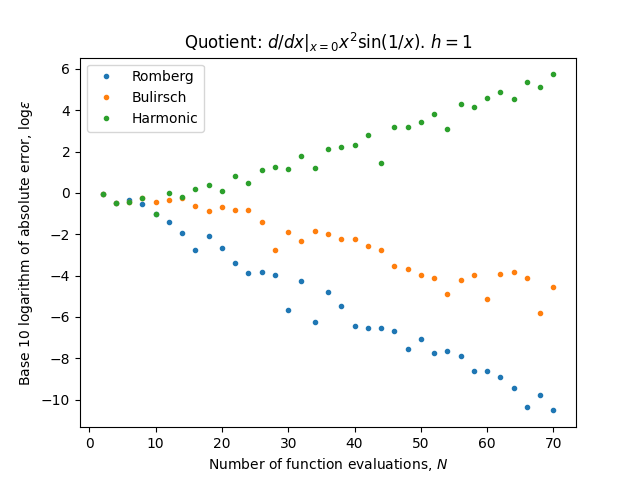
\includegraphics[scale=0.45]{../results/diff_quot_plots/xsin_hp.png}
\end{minipage}
\end{figure}

\begin{figure}[H]
\centering
\begin{minipage}{0.45\textwidth}
\centering
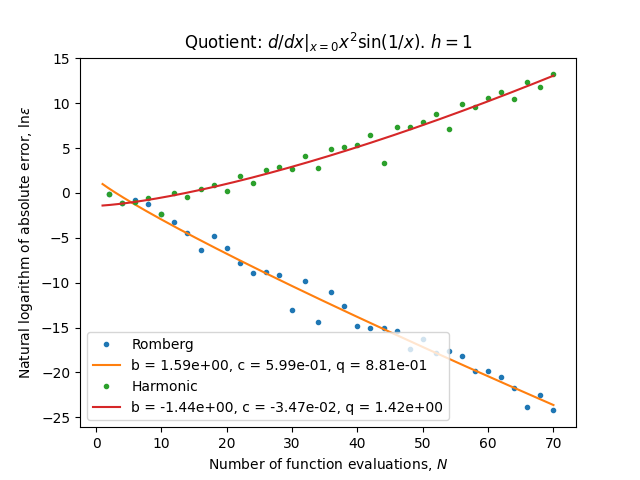
\includegraphics[scale=0.45]{../results/diff_quot_plots/xsin_hp_trend.png}
\end{minipage}
\end{figure}

\begin{table}[H]
    \centering
    \small
    \small
    \begin{tabular}{c||c|c|c|c|c|c|c|c}
Sequence & \(A\)-mean & \(A\)-var & \(c\)-mean & \(c\)-var & \(q\)-mean & \(q\)-var & \(\rho_{\operatorname{lin}}\)& \(\rho_{\ln}\)\\\hline
\rowcolor{red}
RS & \(2.0[+27]\) & \(1.3[+01]\) & \(6.1[+00]\) & \(3.8[+00]\) & \(8.1[-01]\) & \(4.0[-01]\) & \(7.1[-01]\) & \(4.5[-03]\) \\
\rowcolor{red}
HS & \(4.0[-01]\) & \(1.7[+00]\) & \(-3.7[-01]\) & \(6.7[+00]\) & \(1.3[+00]\) & \(9.3[-02]\) & \(9.3[-02]\) & \(1.5[-02]\) \\
    \end{tabular}
    \label{tab:my_label}
\end{table}

Here the model simply does not fit. Note that we do not have the asymptotic expansion for the derivate here, since the function is only once differentiable.\\